\section{Angular Momentum \& Parity}
\subsection{Angular Momentum of the Nucleus}
\begin{itemize}
    \item Total angular momentum $j = l + s$ is the sum of the orbital angular momentum $l$ and the spin $s$. 
    \item Both $l$ and $s$ are quantized, and the total angular momentum $j$ is also quantized.
    \item Nucleons are fermions and therefore spin half particles. 
    \item Fermions can't rotate, but still have spin $s$. There is no classical analogy for this. $l$ is the orbital angular momentum and is just like the classical angular momentum.
\end{itemize}
\subsubsection{Orbital Angular Momentum}
Angular momentum is a vector and thus has both magnitude and direction. As the values are quantized we use the quantum numbers $l$, $s$ and $j$ to describe the magnitude and direction. 
\begin{itemize}
    \item $l$ is the orbital angular momentum and can take the values $0, 1, 2, 3, \ldots$.
    \item Magnitude: 
    \begin{align}
    l &= \sqrt{l(l+1)}ℏ \\
    l_z &= m_lℏ \quad , \quad m_l ∈ \{-l, -l+1, \ldots, l-1, l\} 
    \end{align} 
    \item Direction \cref{fig: angular_momentum_sphere}:
    \begin{figure}[h!]
        \centering
        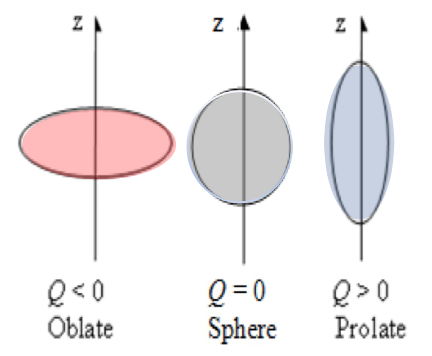
\includegraphics[width = .75\textwidth]{angular_momentum_sphere.png}
        \caption{Orbital angular momentum vector visualized on a sphere.}
        \label{fig: angular_momentum_sphere}
    \end{figure}
\end{itemize}    

\subsubsection{Spin}
\begin{itemize}
    \item Spin is a property of particles and is not related to the motion of the particle. 
    \item Spin is quantized and can take the values $s = \frac{1}{2}$ or $s = -\frac{1}{2}$.
    \item Magnitude: 
    \begin{align}
    s &= \sqrt{s(s+1)}ℏ \\
    s_z &= m_sℏ \quad , \quad m_s ∈ \{-s, -s+1, \ldots, s-1, s\} 
    \end{align} 
    \item As the spin $s$ can only be $1 / 2$, the magnetic quantum number $m_s$ can only be $\pm 1 / 2$
    \item Direction \cref{fig: spin_direction}: There is no classical analogy for direction, but if in a magnetic field, the spin will align with or against the field 
    \begin{figure}[h!]
    \centering
    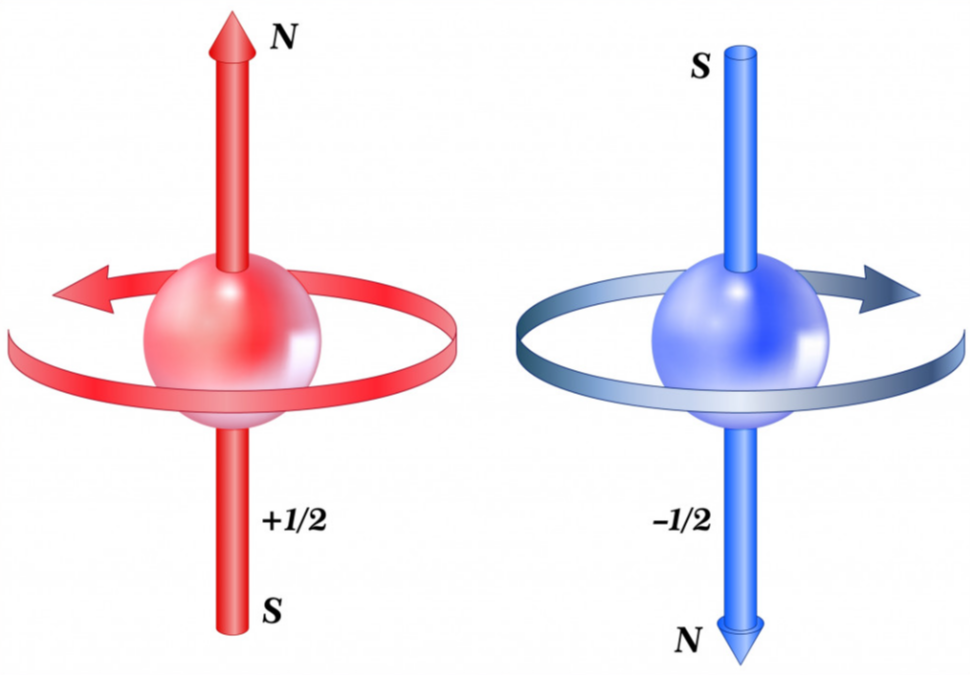
\includegraphics[width = .75\textwidth]{spin_direction.png}
    \caption{Visual representation of the spin of a nucleon in a magnetic field.}
    \label{fig: spin_direction}
    \end{figure}
\end{itemize}
\newpage
\subsubsection{Total Angular Momentum}
\begin{itemize}
    \item The total angular momentum $j$ is the sum of the orbital angular momentum $l$ and the spin $s$.
    \item Magnitude: 
    \begin{align}
    j &= \sqrt{j(j+1)}ℏ \\
    j_z &= m_jℏ \quad , \quad m_j ∈ \{-j, -j+1, \ldots, j-1, j\} \\
    m_j &= m_l + m_s = m_l ± \frac{1}{2}
    \end{align}
    \item Direction \cref{fig: total_angular_momentum_visualized}:
    \begin{figure}[h!]
    \centering
    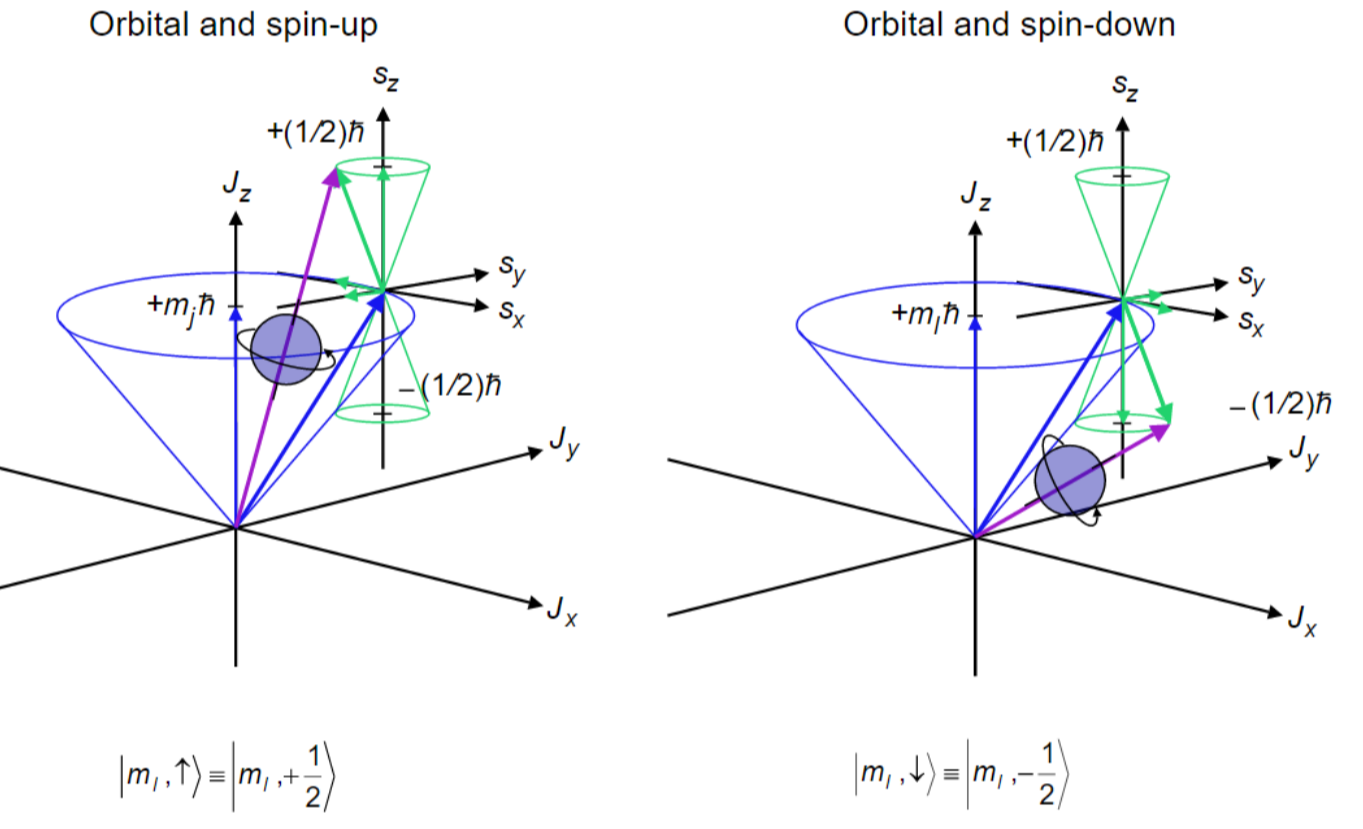
\includegraphics[width = .75\textwidth]{total_angular_momentum_visualized.png}
    \caption{Total angular momentum visualized in 3D.}
    \label{fig: total_angular_momentum_visualized}
    \end{figure}
\end{itemize}

\subsubsection{Total Angular Momentum of the Nucleus}
\begin{itemize}
    \item The sum of the angular momentum of all the nucleons in the nucleus. 
    \begin{align}
    \vec{I} &= \sum_{i=1}^{A} \vec{j}_i \quad , \quad  \vec{j}_i = \vec{l}_i + \vec{s}_i \\
    I &= \sqrt{I(I+1)}ℏ \\
    I_z &= mℏ \quad , \quad m ∈ \{-I, -I+1, \ldots, I-1, I\}
    \end{align} 
    \item As each nucleus has half-integer total angular momentum, odd number of nucleons $A$ will have half-integer total angular momentum, and even number of nucleons will have integer total angular momentum.
    \item All the known even-even nuclei have spin-0 ground states. 
    \item As a result, the ground state of an odd $A$ nucleus must be the $j$-value of the odd proton or neutron. 
\end{itemize}

\subsection{Parity}
Parity is the behavior of a system under the inversion of all spatial coordinates $\vec{r} → - \vec{r}$
\begin{itemize}
    \item Cartesian coordinates: $r → (-x, -y, -z)$. 
    \item Spherical coordinates: $r → (r, π-θ, φ + π)$.
    \item The parity operator is $\hat{P}$ and has two effects on the wave function: 
    \begin{itemize}
        \item Even parity (+): $\hat{P}ψ(\vec{r}) = ψ(\vec{r})$.
        \item Odd parity (-): $\hat{P}ψ(\vec{r}) = -ψ(\vec{r})$.
        \item An even function is symmetric around the origin and an odd function is antisymmetric around the origin. This means $ψ(-r) = ψ(r)$ or $ψ(-r) = -ψ(r)$. 
        \item Visual representation \cref{fig: even_vs_odd_function}:
        \begin{figure}[h!]
        \centering
        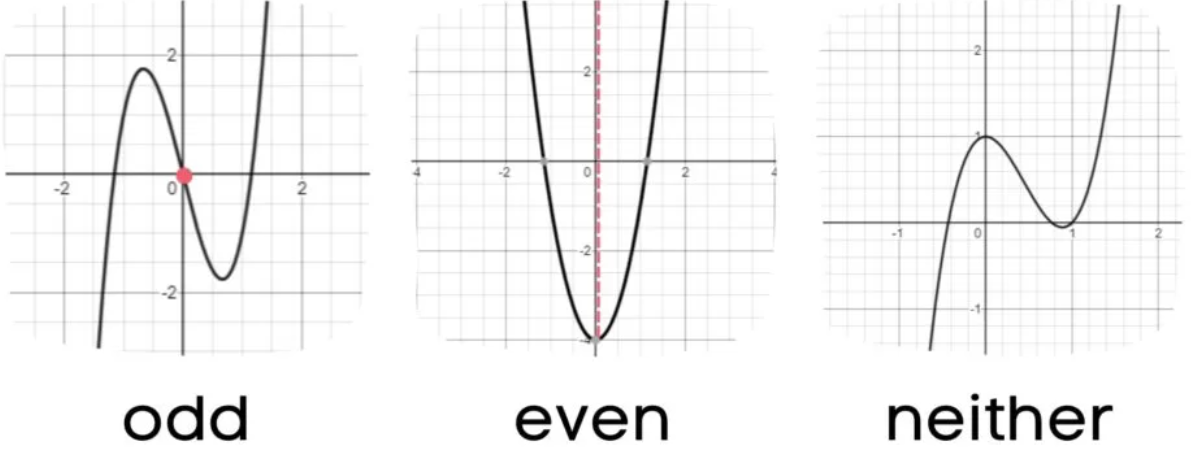
\includegraphics[width = .75\textwidth]{even_vs_odd_function.png}
        \caption{Visual representation of even and odd functions.}
        \label{fig: even_vs_odd_function}
        \end{figure}
    \end{itemize} 
\end{itemize}
\subsubsection{Splitting the Wave Function}
\begin{itemize}
    \item The wave function can be split into its radial and angular parts.
    \begin{align}
    Ψ(\vec{r}) &= R(r)Y(\theta, φ) \\
    \hat{P}R(r) &= R(r) \\
    \hat{P}Y(\theta, φ) &= (-1)^lY_{l}^{m}(θ, ϕ)
    \end{align} 
    \item Parity of state with orbital angular momentum $l$ 
    \begin{equation}
    π(-1)^{l}
    \end{equation} 
    \item By convention, the intrinsic parity of the nucleon is $π = +1$, because they are fermions. Anti-fermions (like positron) have $π = -1$.
    \item For a composite system, the parity is the product of the intrinsic parities of the constituents.
    \begin{equation}
      π_{\text{total}} = (-1)^{L}π_1π_2π_3 \ldots \quad , \quad  L = l_1 + l_2 + l_3 + \ldots
    \end{equation}
\end{itemize}

\section{Electric and Magnetic Moments}
\begin{itemize}
    \item The protons create a magnetic and electric fields. 
    \item A distribution of charge is assigned an electric dipole moment of either monopole, dipole, quadrupole, octopole, etc.
    \item A spherical charge distribution gives only a monopole. 
    \item A circular current only gives a magnetic dipole. 
    \item Nuclei tend to have as simple of dipole moments as possible. 
    \begin{itemize}
        \item L = 0: Monopole
        \item L = 1: Dipole
        \item L = 2: Quadrupole
        \item L = 3: Octopole
    \end{itemize}
\end{itemize}

\subsection{Parity Selection Rules}
\subsubsection{Electric Dipole Moments $E_0$}
\begin{equation}
  L = 0, 2
\end{equation}
Allowed values are $L ∈ {0,2}$ with a parity of $(-1)^{L}$. A dipole is a measure of the separation of positive and negative charge. In the nucleus there is no separation. 

The electric monopole moment is just the charge of the nucleus $Z ⋅ e$.


\subsubsection{Magnetic Dipole Moments $M_1$}
\begin{equation}
  L = 1
\end{equation}
Allowed values are $L = 1$ with a parity of $(-1)^{L+1} = 1$. The magnetic monopole has not been observed. 

As the charged particles are moving, they create a magnetic field. For an electron orbiting a nucleus, we get the following:
\begin{equation}
  \left|\vec{μ}\right| = \frac{e}{2πr / v} πr^2 = \frac{e}{2m}\left|\vec{l}\right|
\end{equation}
This connects the magnetic moment to the mass of the particle. The same goes for the protons in the nucleus. We know the $z$-component of the orbital angular momentum and can be inserted to the equation:
\begin{equation}
  μ = \frac{eℏ}{2m}l
\end{equation}
\subsection{Bohr Magneton \& Nuclear Magneton}
For atomic motion, the electron mass is used.
\begin{align}
μ_{B} = \frac{eℏ}{2m_{e}}  = 5.788 ⋅ 10^{-5} \text{ eV/T}
\end{align}
For nuclear motion, the proton mass is used.
\begin{align}
μ_{N} = \frac{eℏ}{2m_{p}}  = 3.152 ⋅ 10^{-8} \text{ eV/T}
\end{align}

As $μ_{B} ≫ μ_{N}$, the nuclear magnetic moment plays much smaller role in atomic physics.

\subsection{Magnetic Moments of Nuclei}
\begin{itemize}
    \item Magnetic Dipole Moment:
    \begin{itemize}
        \item The magnetic dipole moment of the nucleons is caused by their orbital motion. $μ = g_l μ_{N}l$. 
        \item The g-factor $g_l$ is a dimensionless quantity characterizing the magnetic moment of the atom, nucleus or other particle in question. 
        \item Protons have $g_l = 1$
        \item Neutrons have $g_l = -0.5$. It was believed to be zero, but it proves it's not a point particle.
    \end{itemize}
    \item Spin Magnetic Dipole Moment:
    \begin{itemize}
        \item The magnetic dipole moment of the nucleons is caused by their spin. $μ = g_s μ_{N}s$.
        \item The g-factor $g_s$ is a dimensionless quantity characterizing the magnetic moment of the atom, nucleus or other particle in question.
        \item Protons have $g_s = 5.59 ± 0.0000022$
        \item Neutrons have $g_s = -3.82 ± 0.0000022$. This is unexpected as the neutron is a neutral particle. This shows there charge inside the neutron, and it is not a point particle.
        \item Electrons have $g_s = 2$
    \end{itemize}
\end{itemize}

\subsubsection{Nuclear Structure from Magnetic Moments}
\begin{itemize}
    \item The pairing force favors the coupling of the nucleons such that the sum of their total angular momentum is zero. 
    \item As a result, the magnetic moment of the nucleus is determined by the unpaired nucleons.
    \item Example \cref{fig: nuclear_magnetic_dipole_samples}:
    \begin{figure}[h!]
    \centering
    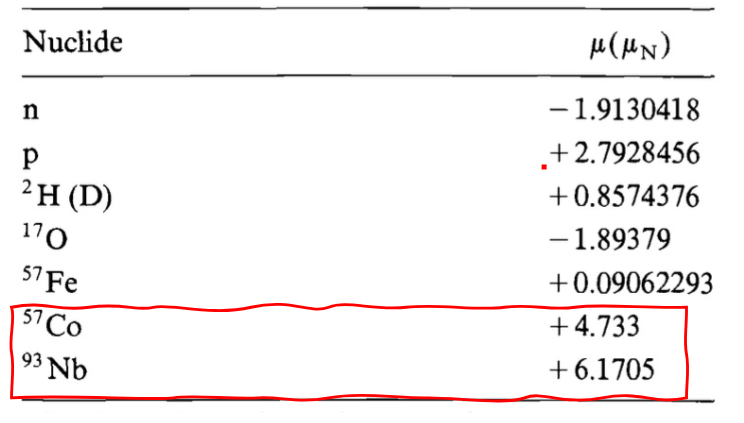
\includegraphics[width = .75\textwidth]{nuclear_magnetic_dipole_samples.png}
    \caption{Table showing the magnetic dipole moments of different nuclei. The box in red shows how larger atoms have a larger magnetic dipole moment, caused by more unpaired nucleons.}
    \label{fig: nuclear_magnetic_dipole_samples}
    \end{figure}
    
\end{itemize}

\subsection{Electric Quadrupole Moments $E_2$ \& Shape of the Nucleus}
Visual representation of the electric quadrupole moments effect on the shape of the nucleus in \cref{fig: nucleus_shape_E2}. 
\begin{equation}
  eQ = e ∫ ψ^{*}(3z^2 - r^2)ψ \ \mathrm{d}v
\end{equation}
Experiment shows that large nuclei like Barium, has a pear-like shape. 
\begin{figure}[h!]
\centering
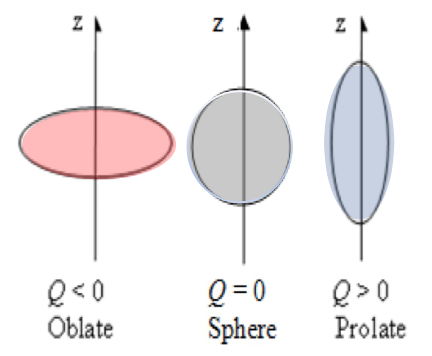
\includegraphics[width = .5\textwidth]{nucleus_shape_E2.png}
\caption{Shape of the nucleus as a function of the electric quadrupole moment.}
\label{fig: nucleus_shape_E2}
\end{figure}

